\documentclass[pdftex,12pt,a4paper]{article}
\usepackage{mathptmx}
\usepackage{blindtext}
\usepackage{graphicx}
\usepackage{subfiles}
\usepackage{amsmath}
\usepackage{amsthm}
\usepackage{tikz}
\usepackage{wrapfig}
\usepackage{lscape}
\usepackage{booktabs}
\usepackage{rotating}
\usepackage{epstopdf}
\usepackage{subcaption}
\usepackage{natbib}
\usepackage[font=small,labelfont=bf]{caption}
\usepackage{hyperref}
\usepackage{color}
\usepackage{algorithm}% http://ctan.org/pkg/algorithms
\usepackage{algpseudocode}% http://ctan.org/pkg/algorithmicx
\hypersetup{
    colorlinks=true,
    linkcolor=blue,
    citecolor=blue
}
\theoremstyle{definition}
\newtheorem{definition}{Definition}[section]
\newtheorem{theorem}{Theorem}[section]
\newtheorem{lemma}[theorem]{Lemma}
\theoremstyle{remark}
\newtheorem*{remark}{Remark}
\usepackage{amssymb}
\usepackage{amsfonts}
\usepackage{mathtools}
\usepackage{geometry}
 \geometry{
 a4paper,
 total={210mm,297mm},
 left=20mm,
 right=20mm,
 top=20mm,
 bottom=20mm,
 }
\renewcommand{\baselinestretch}{2.0}
\newcommand{\defeq}{\vcentcolon=}
\newcommand{\eqdef}{=\vcentcolon}
\newcommand*{\V}[1]{\mathbf{#1}}%
\newcommand{\norm}[1]{\left\lVert#1\right\rVert}
\newcommand{\justif}[2]{&{#1}&\text{#2}}
\newcommand{\qedwhite}{\hfill \ensuremath{\Box}}
\newcommand\given[1][]{\:#1\vert\:}
\newcommand{\me}{\mathrm{e}}
\DeclarePairedDelimiterX{\infdivx}[2]{(}{)}{%
  #1\;\delimsize\|\;#2%
}
\DeclarePairedDelimiter\abs{\lvert}{\rvert}%
\newcommand{\Conv}{\mathop{\scalebox{1.5}{\raisebox{-0.2ex}{$\ast$}}}}%
\newcommand{\infdiv}{\infdivx}
\newcommand\tab[1][1cm]{\hspace*{#1}}
\newcommand{\parder}[2]{\frac{\partial{#1}}{\partial{#2}}}
\renewcommand{\qed}{\hfill\blacksquare}
\hyphenation{op-tical net-works semi-conduc-tor tech-no-lo-gy}



\title{Interpretable Recurrent Neural Network Architectures for Time Series Prediction}
\author{Bernardo P\'erez Orozco}
\date{}
\begin{document}

\maketitle

This report is submitted as part of my Confirmation of Status application, and it accompanies the journal submission \textit{MOrdReD: Memory-based Ordinal Regression Deep Neural Networks for Time Series Forecasting}. Sections 1-4 of this report (which correspond to the second deliverable of the Confirmation of Status written tasks) describe the plan for completion, including an overall description of the thesis, a detailed discussion of specific research projects undertaken, an estimate of the current state of completion of this thesis, and a completion timetable. Section 5 corresponds to the third and final task of the application and replicates form GSO.14.MPLS, which contains a self-assessment of training and development skills acquired over the course.

\section{Outline of overall research contribution}
The principal aim of this DPhil dissertation is to develop a novel Machine Learning time series forecasting framework. There is a very rich literature on time series forecasting tasks, including both Machine Learning methods and others drawn from the classical Statistics corpus. However, several aspects remain either unsolved or with room for improvement.

\subsection{Challenges addressed in this thesis}

\textbf{Autoregressive long-term forecasting.} Whereas regression tasks are traditionally associated with minimising a magnitude deviation metric between forecasts and target variables, decision-makers benefit from having more information than a single point-estimate forecast $\mathbf{\hat{x}}_t$. State-of-the-art forecasting aims to infer model parameters in a Bayesian fashion, i.e. to infer a \textbf{posterior distribution} of the parameters after seeing the available data; and then propagate such uncertainty onto their predictions, which are presented in the form of a \textbf{posterior predictive distribution}. Such densities enable decision-makers to derive confidence intervals, in addition the existence of multiple likely outcomes at the same time instant (i.e. multi-modality). It is thus key that models be able to choose and sequentially adapt the shape of their predictive densities. At present however, state-of-the-art models often assume uni-modal Gaussian predictive likelihoods, which can be regarded as potentially restrictive.

Furthermore, in the setting of long-term forecasting, and particularly that of autoregressive prediction, one additional crucial aspect is that models be able to sequentially forward-propagate forecast uncertainty, i.e. learn an uncertainty growth mechanism as time flows. Failure to do so puts models at risk of becoming overconfident in their predictions and severely underestimating predictive uncertainty. 
    
\textbf{Reliability and honesty.} Mapping predictive densities to real-world probabilities is key \citep{guo2017calibration} if decision-makers are to use this information to solve tasks. Indeed, the degree of correspondence between both is arguably directly proportional to the reliability and usefulness of the entire forecast itself. Evaluating and subsequently adding model calibration strategies is thus an important requirement in the development of time series forecasting frameworks.

\textbf{Feature selection and interpretability.} The Machine Learning literature has historically dealt with developing feature extraction models for a variety of application domains, such as Natural Language Processing. However, one long-standing goal of the field  (and AI in general) is to develop models that can perform automatic salient feature extraction, thus minimising human involvement whilst also trying to avoid a compromise in the interpretability of such representations. 

Feature extraction, as well as data preprocessing methods such as seasonal and linear detrending, in addition to kernel design for models such as Gaussian Processes, are examples of widespread tasks in the time series community in which human intervention may still be required. Automating this process therefore motivates the development of Machine Learning frameworks that can achieve such end-to-end forecasting.

\textbf{Scalability with dataset size.} In the presence of \textit{big data}, we require models that can efficiently learn long-term patterns and tell apart redundancy and noise, without compromising computational complexity in time and memory. At the same time, we require models that can extrapolate and provide accurate uncertainty bounds even from little data. At present, nonparametric statistical models such as Gaussian Processes dominate the time series literature and are known to excel even when there's scarce data availability,  are also known to have difficulties scaling with the size of data.

\subsection{Time series forecasting with recurrent neural networks and ordinal regression}
The first main contribution of this dissertation is the development of a time series framework that addresses the challenges described above. We propose a Memory-based Ordinal Regression Deep neural network (MOrdReD) approach, which conforms the backbone of this dissertation. This framework is described in full detail in the accompanying paper, but we briefly describe how it relates to the aspects described above:

\textbf{Sequential ordinal regression.} This type of task lies between classification and regression. In its simplest version, it consists in quantising the observed time series into a series of bins, which effectively transforms the problem into a sequence learning one, akin to those that frequently arise in the Natural Language Processing literature, but with the crucial difference that the output classes are assumed to have a natural ordering. This simple yet powerful approach enables a number of desirable features: on one hand, it allows the model to represent \underline{rich multi-modal, non-Gaussian behaviour}; on the other, it allows dynamically propose and \underline{adapt the shape} of its predictive posterior through time.

\textbf{Neural network-based.} The Long Short Term Memory (LSTM) is a state-of-the-art model for sequence learning, and it is known to be well-suited for sequence learning tasks, \underline{scaling well with data} even in settings where the sequence symbols are drawn from big alphabets like those that frequently arise in the context of Natural Language processing \citep{Sutskever2014,Xu2014,graves2005}. Furthermore, the attention recently paid to the deep learning community has paid off in terms of quick development of specialised methods, hardware and software. LSTMs thus emerge as natural candidates to handle ordinal regression with very coarse-grained quantisation, thence reducing the representation error induced by this process. This approach also enables us to build an \underline{end-to-end} pipeline that minimises little human intervention.

\textbf{Approximate Bayes via dropout.} Recent developments in the Machine Learning literature have shown how dropout \citep{srivastava2014dropout} can be used in a principled way and further be recast as approximate Bayesian inference. This enables neural network based models to \underline{quantify predictive} \underline{uncertainty} in a principled manner.

The second main contribution of this dissertation, which remains to be completed, addresses the aspects of interpretability, feature selection and forecasting with little data. We note that the number of parameters in neural networks tends to grow rapidly, and this model family is thus prone to overfit in the presence of little data, so addressing this aspect is crucial so as to make our framework of real value. Our current work in progress addresses this by providing a General Unified Model (GUM) which is jointly learnt on a collection of time series drawn from an ample number of sources. Such model is inspired by recent work in Computer Vision pre-trained networks such as VGG Net \cite{Simonyan2015}, which can be ported to specific application domains by means of transfer learning methods. 

\textbf{Grand Unified Model (GUM).} The ultimate goal of such a unified model would be to be capable of \underline{extracting temporal features} that enable forecasting of time series the model has not seen before, or otherwise allow for high-quality forecasting (with respect to state-of-the-art baselines) with little training on the \underline{few available datapoints}. In the next section, we provide evidence of work in progress for this contribution that motivates the feasibility of this approach. 

In summary, this dissertation is composed of two main contributions: our memory-based ordinal regression deep neural network framework, which achieves state-of-the-art performance in a number of time series forecasting tasks and is fully outlined in the accompanying paper; and our Grand Unified Model, which addresses the issues of salient temporal feature extraction and time series forecasting with little data. Detail on both of these contributions is given in the next section. 

\section{Description of research contributions}
A brief description of the research items produced to date is provided below. An additional list of items to be generated by the end of the DPhil is subsequently discussed.

\subsection{Contributions up to date}

\textbf{Framework development.} This is the ordinal regression neural network framework described in the previous section. This is a core component in the dissertation and it is described in full detail in Section 3 of the accompanying paper.

\textbf{Large-scale comparison.} We have extensively benchmarked our framework on 45 datasets against other state-of-the-art and classical time series forecasting methods, including Gaussian Processes and state space autoregression. This comparison encompasses a wide range of metrics to evaluate forecast deviation, uncertainty quantification, uncertainty calibration, etc. The complete comparison is detailed in full in Section 4.1 of the accompanying paper.

\textbf{Time series forecasting in Python.} We have made available a time series forecasting library in Python. On top of adding a high-quality implementation of our method, we also provide an usable interface with other commonly-used forecasting libraries such as GPy, Statsmodels, etc. Forecasting and model comparison tasks can be set in a flexible manner and the library offers a wide range of plotting tools that practitioners often require (quantile-quantile plots, time-indexed predictive densities, etc.). The code is available here: \url{https://github.com/bperezorozco/ordinal_tsf}.

\textbf{Event detection framework.} Some time series contain critical events that occur regularly, but at an uncertain time. Knowing when a time series will reach an optimum is an example of such events. Forecasting \textit{when} these will occur next is a critical task in the time series community. In section 4.2 of our accompanying paper, we describe how our model can be used to tackle such tasks.

\textbf{Multivariate time series forecasting and time-delay univariate forecasting.} This is an extension of our framework to higher-dimensional time series. In this unpublished material, we:
\begin{itemize}
    \item Develop an extension to our MOrdReD framework to perform multivariate time series forecasting.
    \item Assess the performance discrepancy between learning the marginal predictive densities for each channel in the series vs. learning a full joint.
    \item Study the effectiveness of representing the full joint predictive of Multivariate MOrdReD as a Mixture of Gaussians.
    \item Show how this extension can be adapted to help improve forecasting in the univariate case: time-delay MOrdReD. This consists in building a a multivariate time series from a univariate one, in which each channel is given by a lagged version of the original sequence. We provide evidence that this version of MOrdReD can improve predictive performance and is less sensitive to neural network hyperparameters.
\end{itemize}

\subsection{Contributions to be completed}

\textbf{General Unified Model.} The main contribution I will be working on the rest of the year is a General Unified Model for time series forecasting based on MOrdReD. The aim with this project is to optimise a model to extract genetic but salient temporal features from arbitrary time series, in such a way that these can later be used to forecasts sequence that have insufficient data to optimise an instance of MOrdReD by themselves. This is justified by the observation that neural networks overfit quickly when there is little data.

Our preliminary experiment was set up in the following fashion. We first constructed 6 individual ordinal datasets (as described in the accompanying paper) from the time series shown in \ref{fig:ts}, and combined them to form a single ordinal dataset with examples of varied dynamics. Then a single MOrdReD model was fit to this dataset. Crucially, the target variables represent the true next observation for each input subsequence, as opposed to class labels as it would be done in sequence classification tasks. After fitting the model, we used t-SNE \citep{vanDerMaaten2008} to visualise one of the encoder's summary, $\mathbf{C}_0$ (see section 3.1 of accompanying paper) and obtained Figure \ref{fig:tsne}.

From Figure \ref{fig:tsne} we can draw that the model learnt to \textit{cluster} sequences, despite it being blind to the original source of each input sequence. This clustering pattern further hints at how the extracted features could be interpreted by human observers, in relation to the dynamics of the original series. Our aim is to repeat this experiment on a much larger scale (on the order of thousands of time series, for instance drawn from the compilation presented in \citep{Fulcher20130048}) and then devise a scheme to transfer such knowledge of dynamic behaviour onto time series where insufficient data has been provided. This project conforms the second largest contribution of this dissertation.

\begin{figure*}
    \centering
    \begin{subfigure}[b]{0.7\textwidth}
        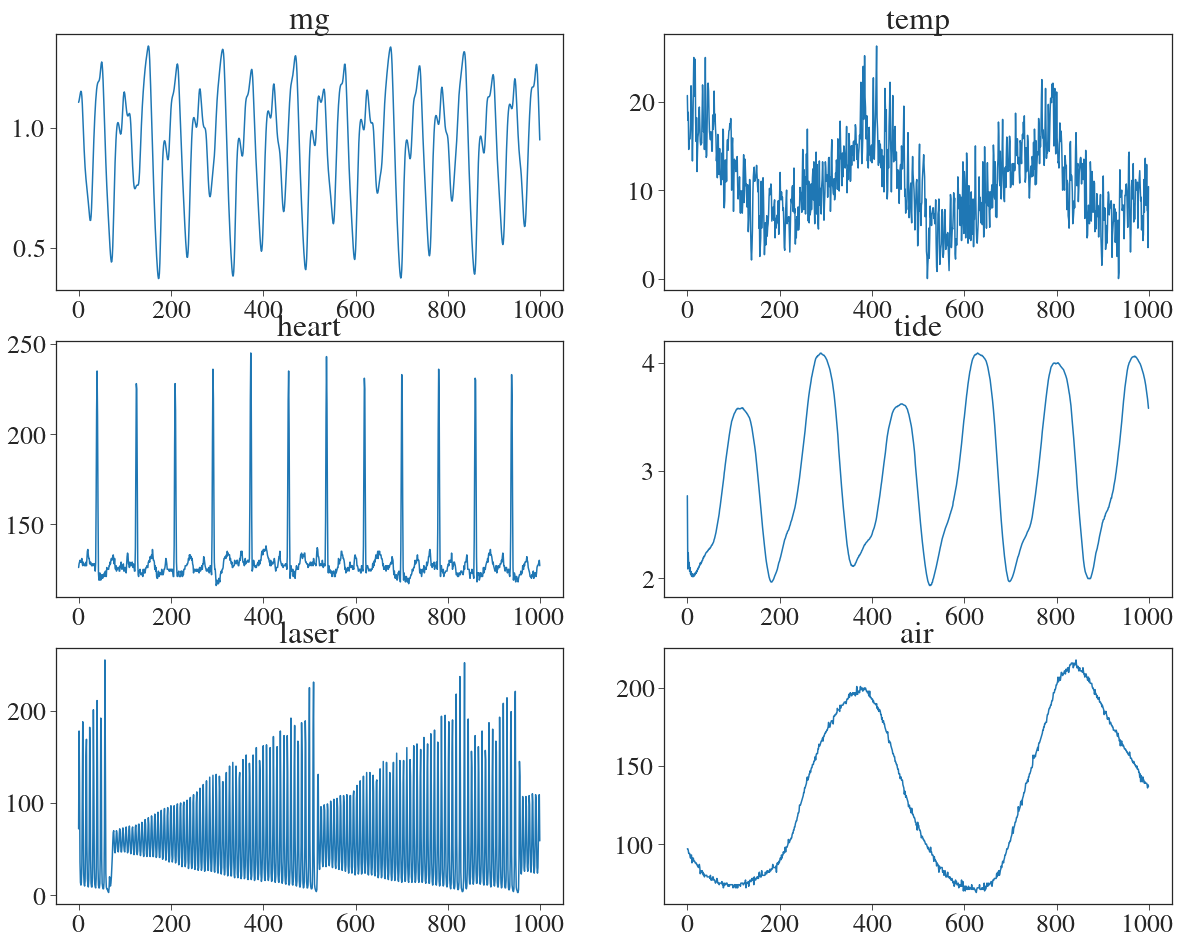
\includegraphics[width=\textwidth]{ts_gum.png}
        \caption{First 1000 observations of the time series used to train our preliminary GUM.}
        \label{fig:ts}
    \end{subfigure}
	
    \begin{subfigure}[b]{0.7\textwidth}
       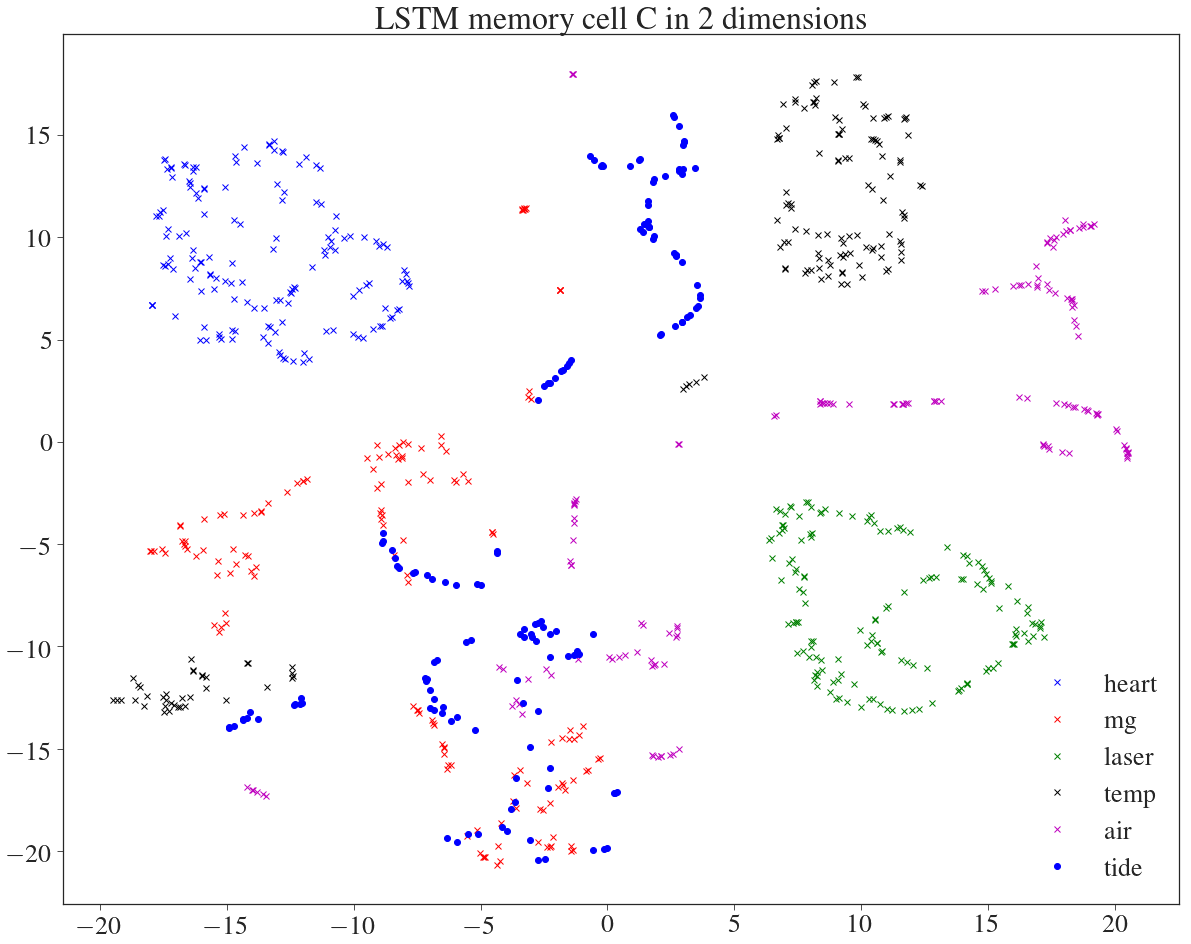
\includegraphics[width=\textwidth]{gumtree_prelim.png}
        \caption{t-SNE feature map obtained from a sequence-to-sequence model's LSTM encoder output trained simultaneously on 6 different time series.}
        \label{fig:tsne}
    \end{subfigure}
	\label{fig:gumtree}
	
	\caption{Time series and extracted features from our preliminary GUM experiment.}
\end{figure*}

\textbf{Case study.} This consists of a detailed example of a real-world time series forecasting task solved with MOrdReD. As opposed to benchmarking our method in a domain-blind fashion, this task involves comparing our performance against other approaches \textit{in the application domain}. This includes benchmarking against approaches that have been recognised in industry and academia for the specific task of interest, and also employing the extensions described so far to incorporate related exogenous time series and other relevant domain knowledge. Previously, due to the authors' previous experience in this domain, this task would consist in forecasting the UK's hourly national solar energy output, as there exist plenty of open available data resources (such as the Met Office's Data Point\footnote{\url{https://www.metoffice.gov.uk/datapoint}} and the University of Sheffield's Sheffield Solar project\footnote{\url{https://www.solar.sheffield.ac.uk/pvlive/}}).


\section{Estimate of current state of completion}
Having described the state of each research item, we now present how these collate as a thesis and the estimated completion percentage of each chapter. Table \ref{tab:completion} presents a summary of the state of affairs.

\begin{table} \centering
\begin{tabular}{lrrrrrr}
\toprule
{Chapter} &     Priority &  Ready to be written &  Weighted completion \\
\midrule
\textbf{1. Introduction} &              5\% &   100\% &            5\% \\
\textbf{2. Background and lit review } &              10\% &   80\% &            8\% \\
\textbf{3. MOrdReD} &              25\% &   100\% &            25\% \\
\textbf{4. MOrdReD extensions} &              15\% &   85\% &            12.75\% \\
\textbf{5. Case study} &              15\% &   25\% &            3.75\%\\
\textbf{6. General Unified Model} &              25\% &   25\% &            6.25\% \\
\textbf{7. Conclusions} &              5\% &   50\% &            2.5\%  \\
\midrule
\textbf{TOTAL} &              100\% &   - &            \textbf{63.25}\%  \\
\bottomrule
\end{tabular}
\caption{Estimated thesis completion. For each chapter, we provide its priority, completion (where 100\% means it is ready to be written) and weighted completion with respect to the thesis.}
\label{tab:completion}
\end{table}

\textbf{Chapter 1. Introduction.} In this chapter, we provide an overview of the time series forecasting task, and then introduce the main contributions of the dissertation.

\textbf{Chapter 2. Background and literature review.} This is an updated version of my transfer of status report. In this chapter we introduce all the needed background to go through the rest of the thesis, crucially concepts such as: ordinal regression, recurrent neural networks, dropout as approximate Bayes, etc.

\textbf{Chapter 3. Memory-based ordinal regression deep neural networks (MOrdReD).} This chapter is largely based on the accompanying journal paper. We introduce our ordinal regression framework and the large-scale benchmarking experiment described in the paper.

\textbf{Chapter 4. MOrdReD extensions.} In this chapter, we describe the MOrdReD extensions we have developed, namely: 
\begin{itemize}
    \item \underline{Multivariate forecasting.} We discuss multivariate forecasting with MOrdReD.
    \item \underline{Time-delay forecasting.} We discuss how univariate forecasting with MOrdReD can be further improved by using its multivariate alternative. This refers to constructing a multivariate series whose every channel is a lagged version of a univariate time series.
    \item \underline{Forecasting event occurrence.} This develops on section 4.2 of the accompanying paper.
    \item \underline{Noise and hyperparameter robustness.} We present our experiments and conclusions on hyperparameter sensitivity and noise robustness.
\end{itemize}

\textbf{Chapter 5. Case study: forecasting energy output in the UK.} As detailed in the previous section, we make a detailed case study in which we benchmark MOrdReD in a specific task against state-of-the-art techniques within a specific application domain. Due to the authors' previous experience with this domain and also due to the availability of open source data, the chosen application domain is that of renewable energy output across the UK.

\textbf{Chapter 6. Towards a General Unified Model.} We introduce the extended General Unified Model described in the previous section, and showcase how this can be applied in the transfer learning setting to do time series forecasting with little data.

\textbf{Chapter 7. Conclusions and future work.} Final remarks and conclusions. 

\section{Completion timetable and risk analysis}
We conclude this report with a detailed timetable of the remaining activities leading to this dissertation's write up, as presented in Figure \ref{fig:timetable}, and a risk assessment. The final submission deadline is Friday of Week 0 Michaelmas Term 2019 at noon. The last 4.5 months before that date are saved up for thesis write-up (3 months) with a slack feedback and corrections (1 month). The months leading to this phase are split among several part-time activities that will be executed in parallel:

\begin{enumerate}
    \item \textbf{MOrdReD paper.} The accompanying paper is currently being submitted to publication, and time has been allocated to deal with reviews and corrections in case of acceptance.
    \item \textbf{General Unified Model.} Being the most ambitious project left to be done, the longest time span has been allocated to it. This project has two subphases: firstly, executing the large-scale model training and hyperparameter tuning, and investigating the extracted temporal features for the training set; subsequently, tuning the model and researching transfer learning and related literature to extrapolate these results to perform time series forecasting on small datasets.
    \item \textbf{MOrdReD extensions.} A number of extensions of our model have been developed and tested. Some time has been allocated to execute more rigorous evaluations on more datasets, and write-up the definitive numbers that will appear in the dissertation.
    \item \textbf{Case study.} This involves acquiring data (including dealing with any external resources we may need to get permission from) and acquiring domain knowledge that may be required to construct the appropriate baselines. Some additional time is allocated for executing the experiments and writing up the final numbers that will appear in the corresponding chapter.
\end{enumerate}

\begin{figure}
    \centerline{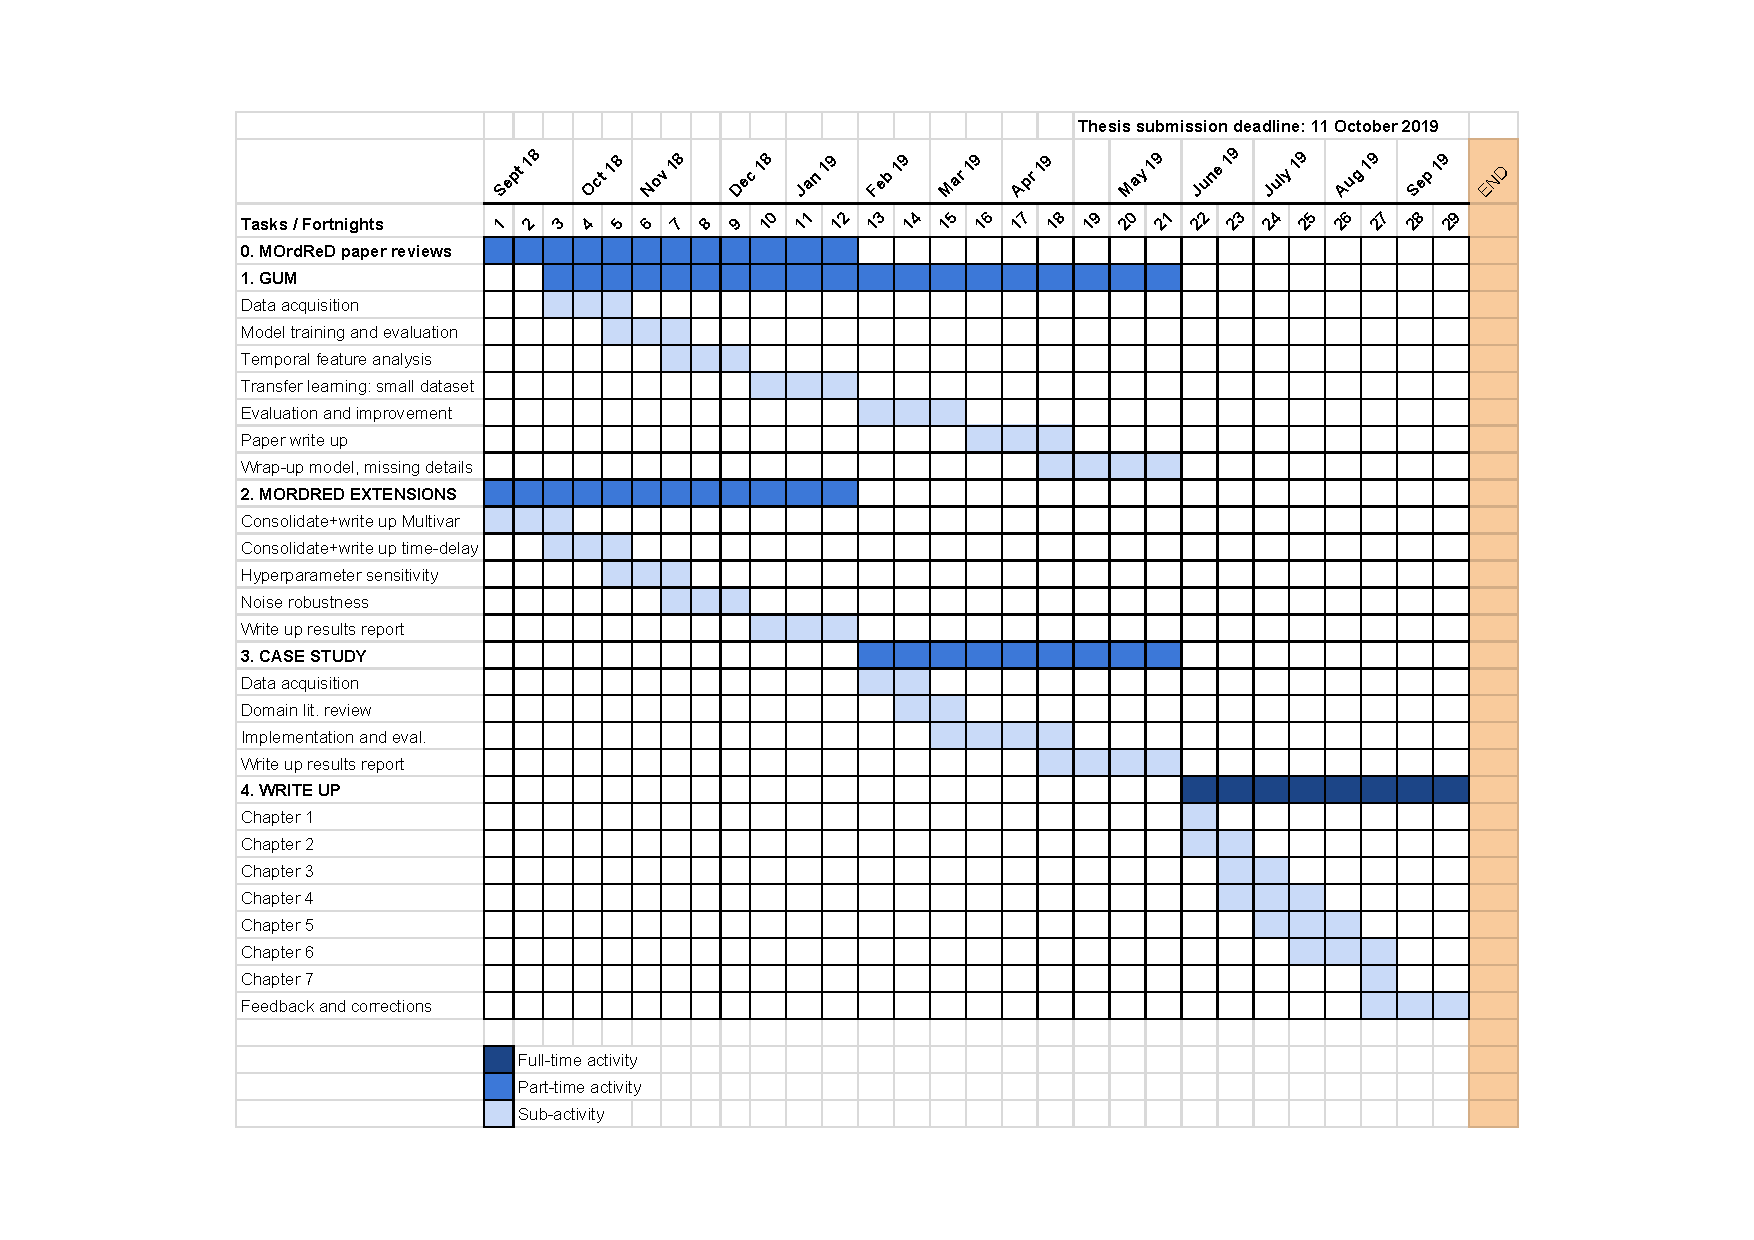
\includegraphics[width=21cm]{CompletionPlan.pdf}}
    \caption{Completion timetable by fortnights and months.}
	\label{fig:timetable}
\end{figure}

The gravest identified risks are the following:
\begin{itemize}
    \item \textbf{Failed paper submission.} One important risk is that the current submission of our journal paper does not go well. If so, more time would need to be allocated to refining this even further (potentially another month), and this could really disrupt the provided timetable. This is being mitigated by polishing as much as possible, and requesting several people for reviews and edits.
    \item \textbf{Unsuccessful General Unified Model.} In this scenario, we find out that the results of this project under-perform, or have little to no impact in comparison with other benchmarks. If this project somehow does not turn into a full contribution that can be added to the thesis, then an additional project of the same weight would need to be designed. On top of making this new idea feel rushed, this scenario could lead to several timetable disruptions. This is being mitigated by prioritising this project and getting results as fast as possible, so this part of the thesis can rest assured.
    \item \textbf{Disrupted timetables lead to funding or visa extensions.} Either of the scenarios above can lead to timetable problems. My funding runs out on September 2019, so any grave disruption to the timetable could lead to extension applications with my sponsor. Furthermore, my visa expires in April 2020, so any extension greater than 6 months could turn into a real problem. This is being mitigated by mitigating the individual risks that could lead to timetable disruptions.  
    \item \textbf{Case study.} The data acquisition step in this phase is critical. Not getting this on time could lead to wholly changing the current choice of application domain, which in turn could translate into timetable disruptions. Whereas not as grave as the previous risks due to the weight of the chapter (Chapter 5) relative to Chapters 3 and 6, this is still a risk to consider.
\end{itemize}

\section{Training and development}
This section is reproduced from the GSO.14.MPLS form submitted alongside this report.

\textbf{1. Please describe briefly any subject specific research skills that you have developed or improved in the course of your time as a research student. For example, these might include: research methodology; data analysis and management; record keeping; bibliographical skills; presentation of research.}
 
During these 9 terms of doctoral research, I have been able to improve my critical understanding of academic publications. This is crucial in spotting strengths and weaknesses of research in the main, and finding areas of improvement for future work.

In terms of research management, I now have clearer ideas and skills on the critical issues of reproducibility and ease of access to research results. In comparison with two years ago, now I feel more careful in terms of guaranteeing I always store intermediate and final results, and in terms of creating generic solutions that can easily be accessed, read and reproduced by anyone in the audience. Such record keeping skills are crucial in areas like Machine Learning, where track needs to be kept for parameters, hyperparameters, plots and even random number generator seeds.

During this last couple of years, we have also made several submissions to Machine Learning conferences. This has undoubtedly helped me to improve my academic writing skills. Evidence of this can be seen in the latest version of our paper in comparison with the very first one some time ago. The improvement in the shape and presentation of this work can be clearly seen.

In addition, I have also had the opportunity to give several presentations, either locally in our group, or as an invited speaker at other universities or groups. This has aided me to improve my oral presentation skills, and importantly being more fluent while giving presentations in English.

Finally, I have also developed skills in data analysis and presentation, crucially gaining a better understanding of visual tools frequently used in the Stati

\textbf{2. Please describe briefly any personal and professional skills in which you have received training or which you have enhanced during the course of your time as a research student. For example, these might include: time management; language skills; IT skills; team work; problem solving; presentation skills; teaching skills; career planning.}

Regarding time management, I have learnt how to better estimate the duration of research activities for better planning. This definitely helps to make realistic plans of what can be achieved under given time frames. I have also managed to consistently maintain a self-managed daily routine, which is a valuable skill to meet deadlines and stick to timetables.

In terms of academic language skills, I feel an improvement not only in how I use the English language, but also in the manner in which I express my ideas in academic documents. One of my first issues in academic writing is a tendency to become very didactic, or struggling to determine the “sweet spot” of when something needs to be explained, and when it can be taken for granted in your audience. Whereas I can still further work on this skill, I definitely sense an improvement in comparison with two years ago.

As for IT skills, I have additionally gained some understanding in an ample set of valuable software packages, such as: Pandas, Keras, Tensorflow, Scikit-learn, GPy, Numpy/Scipy, Statsmodels, etc. This culminated in a time series forecasting Python library I wrote that is now online. 

Regarding teamwork, I can develop on three different axes: the first and most valuable comes from the teamwork I have done with my own supervisor. I work very closely with him and receive valuable feedback. The second axis comes from lab teamwork. I have co-authored two papers with lab peers, which has undoubtedly led to extremely valuable discussions and novel ideas that have been reflected in our research products. The third axis is the experience I received during the internships I did during my PhD. This enabled me to further understand the research environments of industry. Incidentally, this also allowed me to better plan my career ahead, as now I have a clearer idea on the extents in which academia and industry are different, and crucially the pros and cons of each.

In terms of problem solving, thanks to the opportunity I have had to hone my research methodology, I believe I have better, more reasonable approaches to solve problems, in particular in terms of how to approach very open and ill-defined problems.

As for teaching skills, even if I have not taken any teaching seminars again since Year 1, I have had the opportunity to work on this skills through each of the modules I have given in the last two years. More detail on this is given in section D.

\textbf{3. Please identify any subject-specific or personal and professional skills in which you (and your supervisor(s)) foresee the need for further development or training.}

Despite the improvement that I perceive in my writing skills from two years ago, I still feel this is an area of improvement for me. Mainly, I still find myself being too slow when expressing academic ideas in written English. This definitely has an impact on my performance, as I could be spending too much time on tasks that I could otherwise perform faster.

One additional skill I can improve is my fashion of presenting the results of my research. I can still find myself using far-from-ideal plots that are not representative of our results, or not polishing my submissions well enough. I have been working on this skill, but I think improving on this is one priority in this last DPhil year.


\textbf{4. Please list any other activities which have contributed to the development of your work. For example, these might include courses attended, conference presentations given, publications, opportunities to undertake teaching etc.}

Over the last couple of years, I have undertaken two research internships, one at Mind Foundry Ltd. and another one at the Alan Turing Institute. Both of these gave me the opportunity to get a clearer idea of the type of professional career I want to pursue after my DPhil. Crucially, I was able to experience two very different research environments, one from an industrial and another from a rather academic point of view. I also got to experience the type of projects clients in the main are currently interested in, and what kind of methods they use with respect to the standpoint of academia. 

I had a third, part-time position in a slightly different area: public policy at the Mexican Forum of Science and Technology, who are the official source of scientific advice for the Mexican Congress. The main byproduct of this stay was a published article on legislative aspects of AI in developing countries, aimed at Mexican Federal Senators and Deputies. This enabled me to further gain an understanding of other softer aspects of my field, while also allowing me to have a short-term career in scientific public policy, which is an additional professional interest of mine.

I additionally undertook a wide range of teaching activities over the last 9 terms: 
\begin{itemize}
    \item Signal Processing practicals (AIMS CDT): Michaelmas 2016, 2017
    \item Machine Learning practicals (MSc CS): Hilary 2016, Michaelmas 2016, 2017
    \item Tutor for visiting students (Wadham College): Machine Learning (Michaelmas 2016, Trinity 2017), Deep Learning for Natural Language Processing (Hilary 2017), Reinforcement Learning (Trinity 2017)
\end{itemize}

With regard to presentations given, I have been an invited seminar series speaker at the Warwick University Machine Learning Group, in addition to three different seminar tea talks at our own research group.


\bibliographystyle{humannat}
\bibliography{bib}
\end{document}